\documentclass[pdftex,a4paper, 12pt]{article}
%\usepackage{../../support_files/uebungsaufgaben}
\usepackage[utf8]{inputenc}
\usepackage{amsmath}
\usepackage{amsfonts}
\usepackage{amssymb}
\usepackage{graphicx}
\usepackage[usenames,dvipsnames]{color}
% XCOLOR - https://www.latextemplates.com/svgnames-colors
\usepackage[svgnames]{xcolor}
\usepackage{listings}
\usepackage{units}
\usepackage{tikz}
\usepackage[numbers]{natbib}
\usepackage{longtable,tabu}
\bibliographystyle{acm}
%\usepackage[ngerman]{babel}
%par
\setlength{\parindent}{0em}
\setlength{\parskip}{1em}
\usepackage[top=4cm, bottom=3cm, outer=3cm, inner=3cm]{geometry}
%
%
%% common macros
%
\newcommand{\vl}[1]{\mathrm{#1}}    %value
\newcommand{\op}[1]{\mathrm{#1}}	%operator
%
\newcommand{\eg}{e.g. } % e.g.
\newcommand{\ie}{i.e. } % i.e.
%
\newcommand{\eu}{\mathrm{e}}	%Euler number
%
%
%% custom text highlight
\definecolor{mygray}{gray}{0.3}
\newcommand{\highlightg}[1]{\textcolor{mygray}{\bfseries #1}}
%
\date{\today}
\title{Reference model of PEM fuel cell }
\author{Ievgen Golovin, Christian Kunde}
%
%
\begin{document}
%
\maketitle
\tableofcontents
%
%
%\newpage
\section{Introduction}
\label{sec:intro}
%
This documentation presents the reference model of proton exchange membrane (PEM) fuel cell. The model has been proposed in \cite{Mangold2010} and several subsystems have been described in more detail in \cite{Bueck2008, Neubr1999}. In Fig. \ref{fig:scheme} the PEM fuel cell scheme is depicted. From top to bottom this scheme includes the following components: cooling circuit, anode gas channel, anode gas diffusion layer (GDL), anode catalyst layer, membrane, cathode catalyst layer, cathode GDL, cathode gas channel. The electrode of the fuel cell is defined as the assembly of the porous GDL, catalyst layer, and conductor structure. The fuel cell has exactly two electrodes: anode and cathode. They are separated from each other by the ion-conducting membrane. The cell reactions take place on the catalyst layers, and the electrode allows electrons transport through an external circuit.
%
\par
%
The following assumptions are made for the modeling:
%
\begin{itemize}
	\item The model parameters are distributed with respect to the channel direction $z$
	\item Ideal gas model is used to describe behavior of the gases inside the channels and gas diffusion layers
	\item Formation of the liquid water is not considered
	\item Mass and energy are stored in the gas channels
	\item Water is stored in the membrane
	\item Electrodes and current collectors with infinite electrical conductivity are considered
	\item Solid parts (GDLs, catalyst layers, membrane) have one temperature level for each point $z$
\end{itemize}
%
%
\begin{figure}[t]
	\centering
	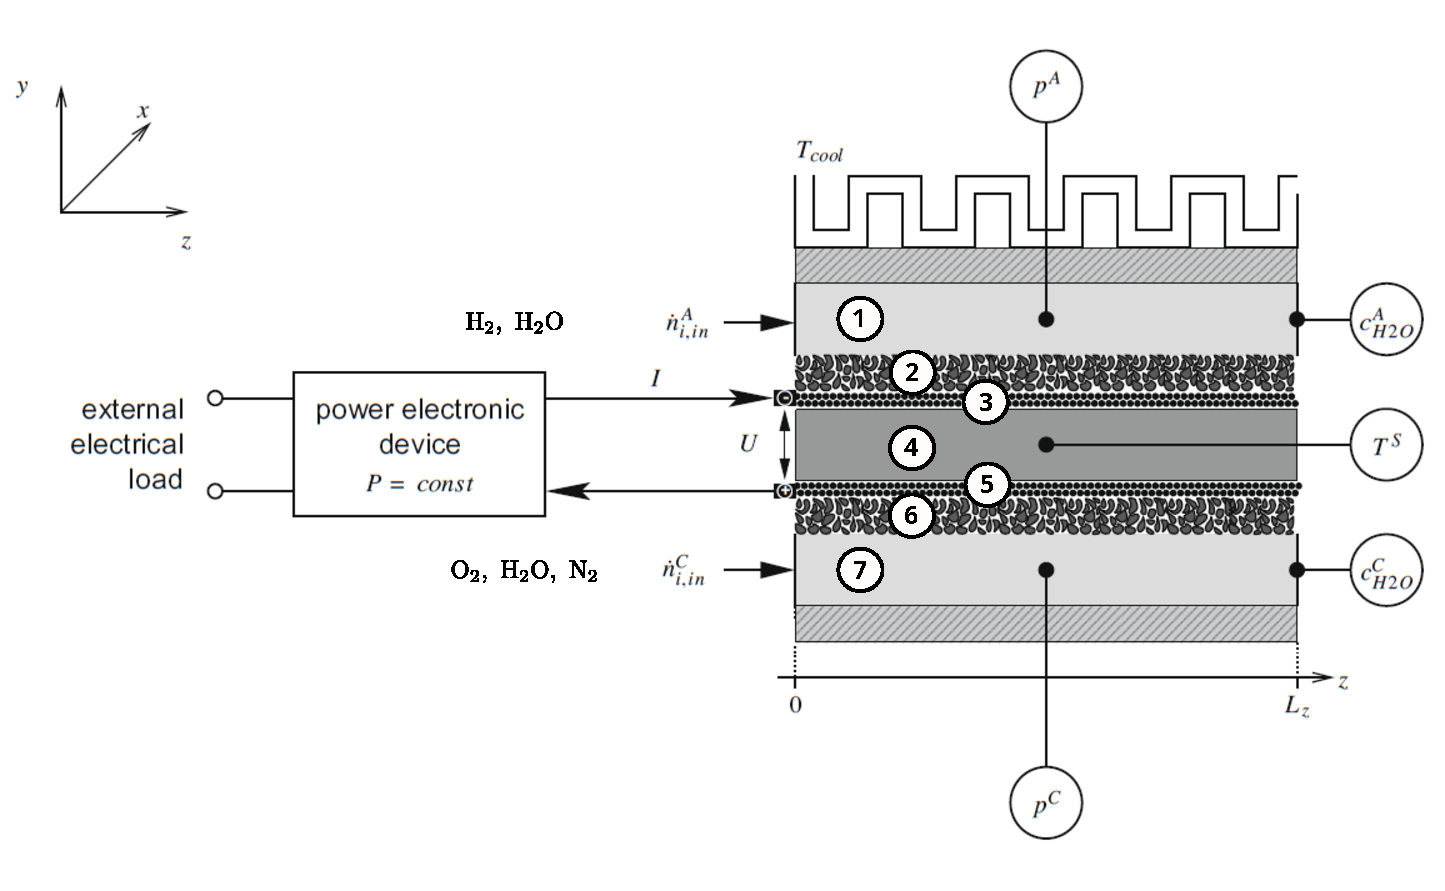
\includegraphics[width=0.95\linewidth]{./figures/pem_fc_scheme.pdf}
	\caption{PEM fuel cell scheme \cite{Mangold2010}}
	\label{fig:scheme}
\end{figure}
%
%
%
Applying these assumptions a distributed parameter model has been obtained. This model is described by nonlinear partial differential equations (PDE) and algebraic equations. For numerical computations the method of lines was applied to the model. The spacial coordinate $z$ was discretized with $N$ finite volumes. This results in the system of nonlinear differential and algebraic equations (DAE):
%
\begin{align}
	\underbrace{\begin{bmatrix} I & 0 \\ 0 & 0 \end{bmatrix}}_{M} \begin{bmatrix} \dot x_{\mathrm{d}} \\ \dot x_{\mathrm{a}} \end{bmatrix} &= \begin{bmatrix}  f(t, 	x_{\mathrm{d}}, x_{\mathrm{a}}, u) \\  g(t, x_{\mathrm{d}}, x_{\mathrm{a}}, u) \end{bmatrix}  
	\label{eq:DAE_sys} \\
	&\Downarrow \nonumber \\
	M \dot{x} &= \tilde{f}(t,x,u) \nonumber
\end{align}
%
with the initial conditions
%
\begin{align}
	x_{\mathrm{d}}(t_0) &= x_{\mathrm{d,0}} 
	\label{eq:DAE_sys_0} \\ 
	g(t_0, x_{\mathrm{d,0}}, x_{\mathrm{a,0}}) &= 0 \nonumber	
\end{align}
%
where the state vector $x$ consists of the dynamic states $x_{\mathrm{d}}$ and algebraic states $x_{\mathrm{a}}$, $u$ is the input vector and $M$ is the corresponding mass matrix.
%
\par
%
%
%
\section{Matlab model overview}
\label{sec:overview}
%
The model (\ref{eq:DAE_sys}), (\ref{eq:DAE_sys_0}) is implemented in Matlab. The model folder has the following directory structure:
%
\begin{itemize}
	\item \texttt{doc/} model documentation
	\item \texttt{res/} MAT-files, e.g. with input trajectory lookup table
	\item \texttt{scr/} model source code
\end{itemize}
%
The model source code folder \texttt{scr/} has the following directory structure:
%
\begin{itemize}
	\item \texttt{scr/data/} add/read/covert external data files  
	\item \texttt{scr/exec/} model script files to run a simulation
	\item \texttt{scr/model/} model functions
	\item \texttt{scr/param/} model parameter structure
	\item \texttt{scr/plotting/} files to plot the results
	\item \texttt{scr/state/} add. functions related to the model system state
	\item \texttt{scr/util/} utility functions
\end{itemize}
%
The model functions folder \texttt{scr/model/} contains the following Matlab functions:
%
\begin{center}
	\begin{tabular}	{p{4.5cm} p{10.5cm}}
		%
		%
		~ & ~ \\
		\texttt{anode\_cat.m} &  anode catalyst layer subsystem \\
		\texttt{anode\_gas\_channel.m} &  anode gas channel subsystem \\
		\texttt{anode\_GDL.m} &  anode GDL subsystem \\
		\texttt{cathode\_cat.m} & cathode catalyst layer subsystem \\
		\texttt{cathode\_gas\_channel.m} & cathode gas channel subsystem \\
		\texttt{cathode\_GDL.m} & cathode GDL subsystem \\
		\texttt{membrane.m} & membrane subsystem \\
		\texttt{ode\_PEMFC.m} & calculates the right hand side $\tilde{f}(t,x,u)$ of (\ref{eq:DAE_sys}) \\
		\texttt{solid\_part.m} & solid subsystem \\
		~ & ~ \\
		%
		%
	\end{tabular}
\end{center}
%
%
The model is computed from \texttt{script\_PEMFC.m}. In this script, solution of DAE problem (\ref{eq:DAE_sys}) using the ode15s-solver is considered. For efficient computations, an additional Jacobian pattern is used. It can be loaded from \texttt{myJPattern.m} function or generated from \texttt{script\_PEMFC.m} (a new one is always needed if the model structure is changed). \\
%
In the current implementation, after the simplification, the following dynamic and algebraic state vectors are used:
%
\begin{align}
	x_{\mathrm{d}} &= \begin{bmatrix} c_{\mathrm{H_2}}^{\mathrm{A}} ~c_{\mathrm{H_2O}}^{\mathrm{A}} ~c_{\mathrm{O_2}}^{\mathrm{C}} ~c_{\mathrm{H_2O}}^{\mathrm{C}} ~c_{\mathrm{N_2}}^{\mathrm{C}} ~\Lambda ~\Delta \mathit{\Phi}^{\mathrm{A}} ~\Delta \mathit{\Phi}^{\mathrm{C}} ~(\rho u)^{\mathrm{A}} ~(\rho u)^{\mathrm{C}} ~(\rho e)^{\mathrm{S}} \end{bmatrix}^T  \in \mathbb{R}^{11} \, ,
	\label{eq:dyn_state_vector} \\
	x_{\mathrm{a}} &= \begin{bmatrix} \xi_{\mathrm{H_2}}^{\mathrm{CA}} ~\xi_{\mathrm{H_2O}}^{\mathrm{CA}} ~\xi_{\mathrm{O_2}}^{\mathrm{CC}} ~\xi_{\mathrm{N_2}}^{\mathrm{CC}} ~\xi_{\mathrm{H_2O}}^{\mathrm{CC}}
		~\Delta \mathit{\Phi}^{\mathrm{M}} ~i^{\mathrm{M}}  ~T^{\mathrm{A}}  ~T^{\mathrm{C}}  ~T^{\mathrm{S}}  ~p^{\mathrm{A}}  ~p^{\mathrm{C}}  ~U_{\mathrm{cell}} \end{bmatrix}^T  \in \mathbb{R}^{13} \, .
	\label{eq:alg_state_vector}
\end{align}
%
The inputs from experimental data are related to the test bench inputs. In order to convert them to the model inputs, i.e.
%
\begin{align}
	u &= \begin{bmatrix} \dot{n}_{\mathrm{H_2,in}}^{\mathrm{A}} ~\dot{n}_{\mathrm{H_2O,in}}^{\mathrm{A}} ~T^{\mathrm{A}}_{\mathrm{in}} ~p^{\mathrm{A}}_{\mathrm{out}} ~\dot{n}_{\mathrm{O_2,in}}^{\mathrm{C}} ~\dot{n}_{\mathrm{H_2O,in}}^{\mathrm{C}} ~\dot{n}_{\mathrm{N_2,in}}^{\mathrm{C}} ~T^{\mathrm{C}}_{\mathrm{in}} ~p^{\mathrm{C}}_{\mathrm{out}} ~T_{\mathrm{cool}} ~I_{\mathrm{cell}} \end{bmatrix}  \, ,
	\label{eq:input_vector}
\end{align}
%
an additional \texttt{testbench2model.m} interface function is used. 
%
\section{Functions and functional subsystems of the model}
\label{sec:fnc}
%
%
The model was implemented in accordance with the equations in \cite{Mangold2010}. The focus of this section is to show equations where approximations or changes have been made. Here, the order of functional subsystems corresponds to Fig. \ref{fig:scheme}. \\
%
For feeding of the gas channels of PEM fuel cells, to strategies can be used:
\begin{enumerate}
	\item co-flow feeding - same directions of flows in the gas channels
	\item counter-flow feeding - opposite directions of flows in the gas channels
\end{enumerate}
In the model it is assumed that the direction of the flow in the anode channel can be changed.
%
\subsection{Anode gas channel}
%
\subsubsection*{Co-flow strategy}
%
The anode gas channel subsystem contains three PDEs that need to be discretized: mass balance, Darcy's law and balance of the internal energy. In order to discretize these PDEs, the finite volume method (FVM) is applied. The application of this method is discussed in detail on the example of mass balance in the anode channel.
%
\subsubsection*{Mass balance}
%
Mass balance in the anode gas channel with corresponding boundary condition can be written as follows:
%
\begin{eqnarray}
	\frac{\partial c_{i}^{\mathrm{A}}(t,z)}{\partial t} &=&-\frac{\partial v^{\mathrm{A}}(t,z) c_{i}^{\mathrm{A}}(t,z)}{\partial z}-\frac{\dot{n}_{i}^{\mathrm{A}}(t,z)}{\delta^{\mathrm{A}}} \, , \label{eq:mass_balA} \\
	\left. v^{\mathrm{A}}(t,z) c_{i}^{\mathrm{A}}(t,z) \right|_{t,0} &=&\dot{n}_{i, \mathrm{\mathrm{in}}}^{\mathrm{A}} \, , \label{eq:mass_balA_bc}
\end{eqnarray}
%
where $i = \mathrm{H_2}, ~\mathrm{H_2O}$.
%
\par
%
For discretization of the PDE with FVM, the spatial coordinate $z$ (see Fig. \ref{fig:scheme}) within the bounds $z_1 = 0$ and $z_{N+1}=L_{z}$ is divided in $N$ control volumes (CV) of equal size and width $\Delta z = L_{z}/N$ as depicted in Fig. \ref{fig:FVM_grid}. The CVs $k = 2,3,\dots,N-1$ are called inner CVs and CVs $k=1$ and $k=N$ are called boundary CVs. The left and right boundary points of each control volume can be defined as
%
%
\begin{eqnarray}
	z_k &=& \Delta z \cdot (k-1) \, , \\
	z_{k+1} &=& \Delta z \cdot k \, .
\end{eqnarray}
%
The nodal points of $k$-th CV follows:
%
\begin{equation}
	z_{\mathrm{m},k} = (z_k + z_{k+1})/2 \, .
\end{equation}  
%
%
\begin{figure}[t]
	\centering
	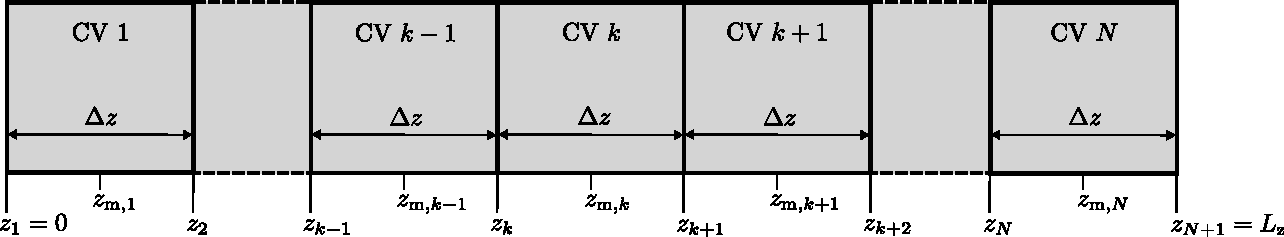
\includegraphics[width=1\textwidth]{./figures/FVM_grid.pdf}
	\caption{Equidistant discretization of the spatial coordinate $z$}
	\label{fig:FVM_grid}
\end{figure}
%
%
At first, PDE (\ref{eq:mass_balA}) is integrated term by term within the boundaries of each inner CV:
%
\begin{eqnarray}
	\underbrace{ \int_{z_k}^{z_{k+1}} \frac{\partial c_{i}^{\mathrm{A}}(t,z)}{\partial t} ~\mathrm{d}z }_{\mathrm{Term~1}} &=& \underbrace{ - \int_{z_k}^{z_{k+1}} \frac{\partial v^{\mathrm{A}}(t,z) c_{i}^{\mathrm{A}}(t,z)}{\partial z} ~\mathrm{d}z }_{\mathrm{Term~2}}  \underbrace{- \int_{z_k}^{z_{k+1}} \frac{\dot{n}_{i}^{\mathrm{A}}(t,z)}{\delta^{\mathrm{A}}} ~\mathrm{d}z }_{\mathrm{Term~3}} \, . \label{eq:mass_balA_int}
\end{eqnarray}
%
%
For integration, a suitable profile assumption has to be made for the integrand terms within the CV. This can be done individually for each term. For boundary CVs, the corresponding boundary conditions have be taken into account.
%
\par
%
For accumulation Term 1 it is assumed that $c_{i}^{\mathrm{A}}(t,z)$ is constant within the $k$-th CV
%
\begin{equation}
	\mathrm{Term~1} = \frac{\mathrm{d}}{\mathrm{d} t} \int_{z_k}^{z_{k+1}}  c_{i}^{\mathrm{A}} ~\mathrm{d}z = \frac{\mathrm{d} c_{i,k}^{\mathrm{A}} }{\mathrm{d} t} (z_{k+1} - z_{k}) = \frac{\mathrm{d} c_{i,k}^{\mathrm{A}} }{\mathrm{d} t} \Delta z  \, .
\end{equation}
%
For convection Term 2 it is assumed that $c_{i}^{\mathrm{A}}(t,z)$ and $v^{\mathrm{A}}(t,z)$ are constant within the $k$-th CV. Taking into account the direction of flux from $k \to k+1$ and corresponding upwind scheme (backward difference), this term can be integrated as follows:
%
\begin{align}
	 \mathrm{Term~2} &=- \int_{z_k}^{z_{k+1}} \frac{\partial v^{\mathrm{A}} c_{i}^{\mathrm{A}}}{\partial z} ~\mathrm{d}z = - \big[ v^{\mathrm{A}} c_{i}^{\mathrm{A}} \big]_{z_k}^{z_{k+1}} = - \big( v_{k}^{\mathrm{A}} c_{i,k}^{\mathrm{A}} - v_{k-1}^{\mathrm{A}} c_{i,k-1}^{\mathrm{A}} \big) \, .
\end{align}
%
For Term 3 it is assumed that $\dot{n}_{i}^{\mathrm{A}}(t,z)$ is constant within the $k$-th CV
%
\begin{equation}
	\mathrm{Term~3} =- \int_{z_k}^{z_{k+1}} \frac{\dot{n}_{i}^{\mathrm{A}}}{\delta^{\mathrm{A}}} ~\mathrm{d}z = \frac{\dot{n}_{i,k}^{\mathrm{A}}}{\delta^{\mathrm{A}}} (z_{k+1} - z_{k}) =  \frac{\dot{n}_{i,k}^{\mathrm{A}}}{\delta^{\mathrm{A}}} \Delta z \, .
\end{equation}
%
Substituting the integrated terms into (\ref{eq:mass_balA_int}) and dividing by $\Delta z$ on both sides, the mass balance in anode gas channel for CVs $k=2 \dots N$ can be obtained
%
\begin{equation}
	\frac{\mathrm{d} c_{i,k}^{\mathrm{A}}}{\mathrm{d} t} =-\frac{v_{k}^{\mathrm{A}} c_{i,k}^{\mathrm{A}} - v_{k-1}^{\mathrm{A}} c_{i,k-1}^{\mathrm{A}}}{\Delta z} - \frac{\dot{n}_{i,k}^{\mathrm{A}}}{\delta^{\mathrm{A}}} \, .
	\label{eq:mass_balA_disc}
\end{equation}
%
%
For CV $k = 1$, boundary condition (\ref{eq:mass_balA_bc}) should be taken into account. Considering the value of the input molar flow, the mass balance for CV 1 follows
%
\begin{equation}
	\frac{\mathrm{d} c_{i,1}^{\mathrm{A}}}{\mathrm{d} t} =-\frac{v_{1}^{\mathrm{A}} c_{i,1}^{\mathrm{A}} - \dot{n}_{i,\mathrm{in}}^{\mathrm{A}} }{\Delta z} - \frac{\dot{n}_{i,1}^{\mathrm{A}}}{\delta^{\mathrm{A}}} \, .
	\label{eq:mass_balA_disc1}
\end{equation}
%
%
\subsubsection*{Darcy's law}
%
%
For Darcy's law it is assumed that $p^{\mathrm{A}}(t,z)$ is constant within the $k$-th CV. Thereafter, the flow velocity can be computed for CVs $k=1 \dots N-1$ applying the forward difference as follows:
%
\begin{equation}
		v_{k}^{\mathrm{A}} = -K^{\mathrm{A}} ~\frac{p_{k+1}^{\mathrm{A}} - p_{k}^{\mathrm{A}}}{\Delta z} \, .
		\label{eq:imp_bal_disc}
\end{equation}
%
For the last volume $N$, the boundary condition has to be taken into account. Considering the value of the pressure at the edge of the last CV and the corresponding distance from the edge to the middle of the CV $0.5 \Delta z$ it follows
%
\begin{equation}
	v_{N}^{\mathrm{A}} = -2 K^{\mathrm{A}} ~\frac{p^{\mathrm{A}}_{\mathrm{out}} - p_{N}^{\mathrm{A}}}{\Delta z} \, .
	\label{eq:imp_bal_discN}
\end{equation}
%
\subsubsection*{Energy balance}
%
Energy balance in the anode gas channel (instead of (7) \cite{Mangold2010}) can be derived as
%
\begin{eqnarray}
	\frac{\partial (\rho u)^{\mathrm{A}}}{\partial t} &=&-\frac{\partial (\rho u v)^{\mathrm{A}}}{\partial z} + \lambda^{\mathrm{A}} 	\frac{\partial^2 T^{\mathrm{A}}}{\partial z^2} + \frac{\alpha_1}{\delta^{\mathrm{A}}} \big( T^{\mathrm{S}} - T^{\mathrm{A}} \big) - \frac{1}{\delta^{\mathrm{A}}} (\rho u v_{\mathrm{y}})^{\mathrm{A}} \, , \label{eq:energy_balA} \\
	(\rho u v)_{\mathrm{in}}^{\mathrm{A}} &=& \left.(\rho u v)^{\mathrm{A}} \right|_{t,0} - \left.\lambda^{\mathrm{A}} \frac{\partial T^{\mathrm{A}}}{\partial z} \right|_{t,0} \, , \label{eq:energy_balA_bc1} \\
	\left.\lambda^{\mathrm{A}} \frac{\partial T^{\mathrm{A}}}{\partial z} \right|_{t,L_{\mathrm{z}}} &=& 0 \, . \label{eq:energy_balA_bc2}
\end{eqnarray}
%
For ideal gas
\begin{eqnarray}
	(\rho u)^{\mathrm{A}} &=& (\rho h)^{\mathrm{A}} - p^{\mathrm{A}} \,\label{eq:rho_u_ideal_gas} \nonumber \\ 
	  &=& \sum_{i} M_{i} c_{i}^{\mathrm{A}} h_{i}(T^{\mathrm{A}}) - R T^{\mathrm{A}} \sum_{i} c_{i}^{\mathrm{A}} \, ,
\end{eqnarray}
%
where $i = \mathrm{H_2}, ~\mathrm{H_2O}$ and enthalpies
%
\begin{equation}
	h_{i}(T) = h_{i}(T_{\mathrm{ref}}) + \int_{T_{\mathrm{ref}}}^{T} c_{\mathrm{p,i}}(T) ~\mathrm{d}T \approx h_{i}(T_{\mathrm{ref}}) + c_{\mathrm{p},i} (T - T_{\mathrm{ref}}) \, .
	\label{eq:enthalpy_gasA}
\end{equation}
%
%
\par
%
For the molar enthalpies it follows
%
\begin{eqnarray}
	(\rho u)^{\mathrm{A}} &=& \sum_{i} c_{i}^{\mathrm{A}} h_{i}(T^{\mathrm{A}}) - R T^{\mathrm{A}} \sum_{i} c_{i}^{\mathrm{A}} \, .
\end{eqnarray}
%
A similar discretization procedure is applied to energy balance PDE. The only difference is the heat conduction term, where the second spatial derivative is present. For this term, it is assumed that the gas temperature $T^{\mathrm{A}}(t,z)$ is linear between two volume nodal points, so that the slope is constant at the volume boundaries of the control volume $k$. For CVs $k=2 \dots N-1$ the energy balance in anode gas channel can be written
%
\begin{align}
	\frac{\mathrm{d} (\rho u)_{k}^{\mathrm{A}}}{\mathrm{d} t} = &-\frac{(\rho u v)_{k}^{\mathrm{A}} 
		- (\rho u v)_{k-1}^{\mathrm{A}} }{\Delta z} 
	 + \lambda^{\mathrm{A}} \frac{T_{k+1}^{\mathrm{A}} -2T_{k}^{\mathrm{A}} +T_{k-1}^{\mathrm{A}}}{\Delta z^2} \nonumber \\ &+ \frac{\alpha_1}{\delta^{\mathrm{A}}} \big( T_{k}^{\mathrm{S}} - T_{k}^{\mathrm{A}} \big) - \frac{1}{\delta^{\mathrm{A}}} \sum_{i} \dot{n}_{i,k}^{\mathrm{A}} h_{i}(T_k^{\mathrm{A}}) + \frac{1}{\delta^{\mathrm{A}}} R T_k^{\mathrm{A}} \sum_{i} \dot{n}_{i,k}^{\mathrm{A}} \, ,
	\label{eq:energy_balA_disc}
\end{align}
%
Discretizing the boundary condition at point $z=0$ (\ref{eq:energy_balA_bc1}) follows
%
\begin{eqnarray}
	(\rho u v)_{0}^{\mathrm{A}} &=& \sum_{i} \dot{n}_{i,\mathrm{in}}^{\mathrm{A}} h_{i}(T_{\mathrm{in}}^{\mathrm{A}}) - R T_{\mathrm{in}}^{\mathrm{A}} \sum_{i} \dot{n}_{i,\mathrm{in}}^{\mathrm{A}} + 2\lambda^{\mathrm{A}} \frac{T_{1}^{\mathrm{A}} - T_{\mathrm{in}}^{\mathrm{A}}}{\Delta z}  \, .
\end{eqnarray}
%
%
Applying the boundary conditions at point $z=0$, the energy balance in anode gas channel for CV $k = 1$ can be written
%
\begin{align}
	\frac{\mathrm{d} (\rho u)_{1}^{\mathrm{A}}}{\mathrm{d} t} = & -\frac{(\rho u v)_{1}^{\mathrm{A}} 
	- (\rho u v)_{0}^{\mathrm{A}} }{\Delta z}
	+ \lambda^{\mathrm{A}} \frac{T_{2}^{\mathrm{A}} - 3 T_{1}^{\mathrm{A}} +2 T_{\mathrm{in}}^{\mathrm{A}}}{\Delta z^2}  \nonumber \\ &+ \frac{\alpha_1}{\delta^{\mathrm{A}}} \big( T_{1}^{\mathrm{S}} - T_{1}^{\mathrm{A}} \big) - \frac{1}{\delta^{\mathrm{A}}} \sum_{i} \dot{n}_{i,1}^{\mathrm{A}} h_{i}(T_1^{\mathrm{A}}) + \frac{1}{\delta^{\mathrm{A}}} R T_1^{\mathrm{A}} \sum_{i} \dot{n}_{i,1}^{\mathrm{A}} \, .
	\label{eq:energy_balA_disc1}
\end{align}
%
Applying the boundary conditions at point $z=L_{z}$, the energy balance in anode gas channel for CV $k = N$ can be written
%
\begin{align}
	\frac{\mathrm{d} (\rho u)_{N}^{\mathrm{A}}}{\mathrm{d} t} = & - \frac{(\rho u v)_{N}^{\mathrm{A}} 
	- (\rho u v)_{N-1}^{\mathrm{A}} }{\Delta z}
	+ \lambda^{\mathrm{A}} \frac{T_{N-1}^{\mathrm{A}} - T_{N}^{\mathrm{A}}}{\Delta z^2}  \nonumber \\ &+ \frac{\alpha_1}{\delta^{\mathrm{A}}} \big( T_{N}^{\mathrm{S}} - T_{N}^{\mathrm{A}} \big) - \frac{1}{\delta^{\mathrm{A}}} \sum_{i} \dot{n}_{i,N}^{\mathrm{A}} h_{i}(T_N^{\mathrm{A}}) + \frac{1}{\delta^{\mathrm{A}}} R T_N^{\mathrm{A}} \sum_{i} \dot{n}_{i,N}^{\mathrm{A}} \, .
	\label{eq:energy_balA_discN}
\end{align}
%
\subsubsection*{Counter-flow strategy}
%
Assuming that the direction of flux from $k+1 \to k$ (see Fig. \ref{fig:FVM_grid}), the same discretization procedure using the FVM is applied. Three PDEs that need to be discretized applying this assumption: mass balance, Darcy's law and balance of the internal energy.
%
\subsubsection*{Mass balance}
%
For CVs $k=1 \dots N-1$, the discretized mass balance equation in the anode gas channel with counter-flow direction can be obtained
%
\begin{equation}
	\frac{\mathrm{d} c_{i,k}^{\mathrm{A}}}{\mathrm{d} t} =-\frac{v_{k}^{\mathrm{A}} c_{i,k}^{\mathrm{A}} - v_{k+1}^{\mathrm{A}} c_{i,k+1}^{\mathrm{A}}}{\Delta z} - \frac{\dot{n}_{i,k}^{\mathrm{A}}}{\delta^{\mathrm{A}}} \, .
	\label{eq:mass_balA_disc_counter}
\end{equation}
%
%
For CV $k = N$, a boundary condition should be taken into account. Considering the value of the input molar flow, the mass balance for CV $N$ follows
%
\begin{equation}
	\frac{\mathrm{d} c_{i,N}^{\mathrm{A}}}{\mathrm{d} t} =-\frac{v_{N}^{\mathrm{A}} c_{i,N}^{\mathrm{A}} - \dot{n}_{i,\mathrm{in}}^{\mathrm{A}} }{\Delta z} - \frac{\dot{n}_{i,N}^{\mathrm{A}}}{\delta^{\mathrm{A}}} \, .
	\label{eq:mass_balA_disc1_counter}
\end{equation}
%
\subsubsection*{Darcy's law}
%
The flow velocity can be computed for CVs $k=2 \dots N$ according to Darcy's law as follows:
%
\begin{equation}
	v_{k}^{\mathrm{A}} = -K^{\mathrm{A}} ~\frac{p_{k-1}^{\mathrm{A}} - p_{k}^{\mathrm{A}}}{\Delta z} \, .
	\label{eq:imp_bal_disc_count}
\end{equation}
%
For CV $k = 1$ it follows
%
\begin{equation}
	v_{1}^{\mathrm{A}} = -2 K^{\mathrm{A}} ~\frac{p^{\mathrm{A}}_{\mathrm{out}} - p_{1}^{\mathrm{A}}}{\Delta z} \, .
	\label{eq:imp_bal_discN_count}
\end{equation}
%
\subsubsection*{Energy balance}
%
%
For CVs $k=2 \dots N-1$ the energy balance in anode gas channel can be written
%
\begin{align}
	\frac{\mathrm{d} (\rho u)_{k}^{\mathrm{A}}}{\mathrm{d} t} = &-\frac{(\rho u v)_{k}^{\mathrm{A}} 
		- (\rho u v)_{k+1}^{\mathrm{A}} }{\Delta z} 
	+ \lambda^{\mathrm{A}} \frac{T_{k-1}^{\mathrm{A}} -2T_{k}^{\mathrm{A}} +T_{k+1}^{\mathrm{A}}}{\Delta z^2} \nonumber \\ &+ \frac{\alpha_1}{\delta^{\mathrm{A}}} \big( T_{k}^{\mathrm{S}} - T_{k}^{\mathrm{A}} \big) - \frac{1}{\delta^{\mathrm{A}}} \sum_{i} \dot{n}_{i,k}^{\mathrm{A}} h_{i}(T_k^{\mathrm{A}}) + \frac{1}{\delta^{\mathrm{A}}} R T_k^{\mathrm{A}} \sum_{i} \dot{n}_{i,k}^{\mathrm{A}} \, .
	\label{eq:energy_balA_disc_count}
\end{align}
%
Discretizing the boundary condition at point $z=L_{z}$ follows
%
\begin{eqnarray}
	(\rho u v)_{\mathrm{in}}^{\mathrm{A}} &=& \sum_{i} \dot{n}_{i,\mathrm{in}}^{\mathrm{A}} h_{i}(T_{\mathrm{in}}^{\mathrm{A}}) - R T_{\mathrm{in}}^{\mathrm{A}} \sum_{i} \dot{n}_{i,\mathrm{in}}^{\mathrm{A}} + 2\lambda^{\mathrm{A}} \frac{T_{N}^{\mathrm{A}} - T_{\mathrm{in}}^{\mathrm{A}}}{\Delta z}  \, .
\end{eqnarray}
%
%
Applying the boundary conditions at point $z=L_{z}$, the energy balance in anode gas channel for CV $k = N$ can be written
%
\begin{align}
	\frac{\mathrm{d} (\rho u)_{N}^{\mathrm{A}}}{\mathrm{d} t} = & -\frac{(\rho u v)_{N}^{\mathrm{A}} 
		- (\rho u v)_{in}^{\mathrm{A}} }{\Delta z}
	+ \lambda^{\mathrm{A}} \frac{T_{N-1}^{\mathrm{A}} - 3 T_{N}^{\mathrm{A}} +2 T_{\mathrm{in}}^{\mathrm{A}}}{\Delta z^2}  \nonumber \\ &+ \frac{\alpha_1}{\delta^{\mathrm{A}}} \big( T_{N}^{\mathrm{S}} - T_{N}^{\mathrm{A}} \big) - \frac{1}{\delta^{\mathrm{A}}} \sum_{i} \dot{n}_{i,N}^{\mathrm{A}} h_{i}(T_N^{\mathrm{A}}) + \frac{1}{\delta^{\mathrm{A}}} R T_N^{\mathrm{A}} \sum_{i} \dot{n}_{i,N}^{\mathrm{A}} \, .
	\label{eq:energy_balA_disc1_count}
\end{align}
%
Applying the boundary conditions at point $z=0$, the energy balance in anode gas channel for CV $k = 1$ can be written
%
\begin{align}
	\frac{\mathrm{d} (\rho u)_{1}^{\mathrm{A}}}{\mathrm{d} t} = & - \frac{(\rho u v)_{1}^{\mathrm{A}} 
		- (\rho u v)_{2}^{\mathrm{A}} }{\Delta z}
	+ \lambda^{\mathrm{A}} \frac{T_{2}^{\mathrm{A}} - T_{1}^{\mathrm{A}}}{\Delta z^2}  \nonumber \\ &+ \frac{\alpha_1}{\delta^{\mathrm{A}}} \big( T_{1}^{\mathrm{S}} - T_{1}^{\mathrm{A}} \big) - \frac{1}{\delta^{\mathrm{A}}} \sum_{i} \dot{n}_{i,1}^{\mathrm{A}} h_{i}(T_1^{\mathrm{A}}) + \frac{1}{\delta^{\mathrm{A}}} R T_1^{\mathrm{A}} \sum_{i} \dot{n}_{i,1}^{\mathrm{A}} \, .
	\label{eq:energy_balA_discN_count}
\end{align}
%
\subsection{Anode GDL}
%
According to \cite{Mangold2010}.
%
%
%
\subsection{Anode catalyst layer}
%
%
In the model, the following anodic reaction rate is used
%
\begin{eqnarray}
	r^{\mathrm{A}} &=& f^{\mathrm{V}} \frac{ i_{\mathrm{A 0}} }{ 2 F} \Big[ \exp \Big( \alpha^{\mathrm{A}} \frac{2 F}{R T^{\mathrm{S}}} \big( \Delta \mathit{\Phi}^{\mathrm{A}} - \Delta \mathit{\Phi}_{\mathrm{ref}}^{\mathrm{A}} \big)\Big) \frac{\xi_{\mathrm{H}_{2}}^{\mathrm{CA}} p^{\mathrm{A}}}{p_{\mathrm{H}_{2}, \mathrm{ref}}} \nonumber \\ 
	&&- \exp \Big( -(1-\alpha^{\mathrm{A}}) \frac{2 F}{R T^{\mathrm{S}}} \big( \Delta \mathit{\Phi}^{\mathrm{A}} - \Delta \mathit{\Phi}_{\mathrm{ref}}^{\mathrm{A}} \big) \Big) \Big] \, .
\end{eqnarray}
%
%
\subsection{Membrane subsystem}
%
\subsubsection*{Water balance in membrane}
%
Water balance in membrane is given by
%
\begin{equation}
	\frac{\partial c_{\mathrm{H_2O}}^{\mathrm{M}}}{\partial t} =\frac{1}{\delta^{\mathrm{M}}}\left(\dot{n}_{\mathrm{H}_{2} \mathrm{O}}^{\mathrm{A M}}+\dot{n}_{\mathrm{H}_{2} \mathrm{O}}^{\mathrm{C M}}\right) \, ,
	\label{eq:membr_bal}
\end{equation}
%
where $c_{\mathrm{H_2O}}^{\mathrm{M}} = \mathit{\Lambda} \rho^{\mathrm{M}}(\mathit{\Lambda}) X^{\mathrm{M}}(\mathit{\Lambda})$.
%
\par
%
Substituting the water concentration $c_{\mathrm{H_2O}}^{\mathrm{M}}$ and reformulating gives
%
\begin{align}
	\frac{\partial \mathit{\Lambda} \rho^{\mathrm{M}}(\mathit{\Lambda}) X^{\mathrm{M}}(\mathit{\Lambda})}{\partial t} =\frac{1}{\delta^{\mathrm{M}}}\left(\dot{n}_{\mathrm{H}_{2} \mathrm{O}}^{\mathrm{A M}}+\dot{n}_{\mathrm{H}_{2} \mathrm{O}}^{\mathrm{C M}}\right) \, ,\\
	\mathit{\Lambda} \frac{\partial \rho^{\mathrm{M}}(\mathit{\Lambda}) X^{\mathrm{M}}(\mathit{\Lambda})}{\partial t} + \rho^{\mathrm{M}}(\mathit{\Lambda}) X^{\mathrm{M}}(\mathit{\Lambda}) \frac{\partial \mathit{\Lambda}}{\partial t} =\frac{1}{\delta^{\mathrm{M}}}\left(\dot{n}_{\mathrm{H}_{2} \mathrm{O}}^{\mathrm{A M}}+\dot{n}_{\mathrm{H}_{2} \mathrm{O}}^{\mathrm{C M}}\right) \, ,\\
	\mathit{\Lambda} \frac{\partial \rho^{\mathrm{M}}(\mathit{\Lambda}) X^{\mathrm{M}}(\mathit{\Lambda})}{\partial \mathit{\Lambda}} \frac{\partial \mathit{\Lambda}}{\partial t} + \rho^{\mathrm{M}}(\mathit{\Lambda}) X^{\mathrm{M}}(\mathit{\Lambda}) \frac{\partial \mathit{\Lambda}}{\partial t} =\frac{1}{\delta^{\mathrm{M}}}\left(\dot{n}_{\mathrm{H}_{2} \mathrm{O}}^{\mathrm{A M}}+\dot{n}_{\mathrm{H}_{2} \mathrm{O}}^{\mathrm{C M}}\right) \, ,\\
	\left( \mathit{\Lambda} \frac{\partial \rho^{\mathrm{M}}(\mathit{\Lambda}) X^{\mathrm{M}}(\mathit{\Lambda})}{\partial \mathit{\Lambda}}  + \rho^{\mathrm{M}}(\mathit{\Lambda}) X^{\mathrm{M}}(\mathit{\Lambda}) \right) \frac{\partial \mathit{\Lambda}}{\partial t} =\frac{1}{\delta^{\mathrm{M}}}\left(\dot{n}_{\mathrm{H}_{2} \mathrm{O}}^{\mathrm{A M}}+\dot{n}_{\mathrm{H}_{2} \mathrm{O}}^{\mathrm{C M}}\right) \, .
\end{align}
% As the product $\rho^{\mathrm{M}}(\mathit{\Lambda}) X^{\mathrm{M}}(\mathit{\Lambda})$ is approximately constant for a wide range of $\mathit{\Lambda}$, the water balance (\ref{eq:membr_bal}) can be simplified as
% %
% \begin{equation}
% 	\rho^{\mathrm{M}}(\mathit{\Lambda}) X^{\mathrm{M}}(\mathit{\Lambda}) \frac{\partial \mathit{\Lambda}}{\partial t}=\frac{1}{\delta^{\mathrm{M}}}\left(\dot{n}_{\mathrm{H}_{2} \mathrm{O}}^{\mathrm{A M}}+\dot{n}_{\mathrm{H}_{2} \mathrm{O}}^{\mathrm{C M}}\right) \, .
% \end{equation}
%
%
\subsubsection*{Sorption isotherm}
%
%
The sorption isotherm provides the determination of the liquid water content at the membrane edges $\mathit{\Lambda}^{\mathrm{AM}}$ and $\mathit{\Lambda}^{\mathrm{CM}}$ from the concentrations of the gaseous water in the catalyst layers. The sorption depends on the relation of the partial pressure of the gaseous water to the saturation pressure at the given temperature
%
\begin{equation}
	a_{\mathrm{H_2O}}^{j} = \frac{p_{\mathrm{H_2O}}^{\mathrm{C}j}}{p_{\mathrm{H_2O}}^{\mathrm{sat}}(\theta)} \, ,
\end{equation}
%
where
%
\begin{align}
	p_{\mathrm{H_2O}}^{\mathrm{sat}} &= 100 \exp{\Big( 19.016 - \frac{4064.95}{\theta + 236.25} \Big)} \, , \\
	\theta ~^{\circ} \mathrm{C} &= T^{\mathrm{S}} - 273.15 ~\mathrm{K} \, .
\end{align}
%
The water contents is fitted for two temperature points $\theta = 30 ~^{\circ} \mathrm{C}$ and $\theta = 80 ~^{\circ} \mathrm{C}$ as follows:
%
\begin{align}
	\mathit{\Lambda}_{30} &= 36 ~a_{\mathrm{H_2O}}^3 - 39.85 ~a_{\mathrm{H_2O}}^2 + 17.81 ~a_{\mathrm{H_2O}} + 0.043 \, , \\
	\mathit{\Lambda}_{80} &= 14.1 ~a_{\mathrm{H_2O}}^3 - 16 ~a_{\mathrm{H_2O}}^2 + 10.8 ~a_{\mathrm{H_2O}} + 0.3 \, .
\end{align}
%
For temperatures between these two curves, the value of the water content is linearly interpolated.
%
%
\subsubsection*{Water transport}
%
According to (28) \cite{Mangold2010} the water transport through the membrane is given by
%
\begin{align}
	\dot{n}_{\mathrm{H_2O}}^j &= - \frac{t_\mathrm{W}(\mathit{\Lambda}) \kappa(\mathit{\Lambda})}{\mathrm{F}^2} (\nabla\mu_{\mathrm{H+}})^j - \frac{D_\mathrm{W}(\mathit{\Lambda}) c_{\mathrm{H_2O}}^\mathrm{M}}{\mathrm{R}T^{\mathrm{S}}} (\nabla\mu_{\mathrm{H_2O}})^j \, ,
\end{align}
%
where $j=\mathrm{AM},\mathrm{CM}$ and
%
\begin{align}
	(\nabla\mu_{\mathrm{H+}})^j &= \mathrm{R}T^{\mathrm{S}} \frac{1}{\xi_{\mathrm{H+}}}(\nabla\xi_{\mathrm{H+}})^j+\mathrm{F}(\nabla\mathit{\Phi})^j \, , \\
	(\nabla\mu_{\mathrm{H_2O}})^j &= \mathrm{R}T^{\mathrm{S}} \frac{1}{\xi_{\mathrm{H_2O}}}(\nabla\xi_{\mathrm{H_2O}})^j \, .
\end{align}
%
\par
%
Adding an additional point for the water concentration in the middle of membrane M, the gradients can be approximated as follows:
%
\begin{align}
	% xi
	\left(\frac{1}{\xi_{\mathrm{H+}}}\nabla\xi_{\mathrm{H+}}\right)^\mathrm{AM} &\approx \frac{2}{ \xi_{\mathrm{H+}}(\mathit{\Lambda}^{\mathrm{CM}})+\xi_{\mathrm{H+}}(\mathit{\Lambda}^{\mathrm{AM}}) } \frac{\xi_{\mathrm{H+}}(\mathit{\Lambda}^{\mathrm{CM}})-\xi_{\mathrm{H+}}(\mathit{\Lambda}^{\mathrm{AM}})}{\delta^{\mathrm{M}}} \, , \\
	% xi
	\left(\frac{1}{\xi_{\mathrm{H+}}}\nabla\xi_{\mathrm{H+}}\right)^\mathrm{CM} &\approx \frac{2}{ \xi_{\mathrm{H+}}(\mathit{\Lambda}^{\mathrm{CM}})+\xi_{\mathrm{H+}}(\mathit{\Lambda}^{\mathrm{AM}}) } \frac{\xi_{\mathrm{H+}}(\mathit{\Lambda}^{\mathrm{AM}})-\xi_{\mathrm{H+}}(\mathit{\Lambda}^{\mathrm{CM}})}{\delta^{\mathrm{M}}} \, , \\
	% xi
	\left(\frac{1}{\xi_{\mathrm{H_2O}}}\nabla\xi_{\mathrm{H_2O}}\right)^\mathrm{AM} &\approx \frac{1}{ \xi_{\mathrm{H_2O}}(\mathit{\Lambda}^{\mathrm{M}}) } \frac{\xi_{\mathrm{H_2O}}(\mathit{\Lambda}^{\mathrm{M}})-\xi_{\mathrm{H_2O}}(\mathit{\Lambda}^{\mathrm{AM}})}{0.5\delta^{\mathrm{M}}} \, ,\\
	% xi
	\left(\frac{1}{\xi_{\mathrm{H_2O}}}\nabla\xi_{\mathrm{H_2O}}\right)^\mathrm{CM} &\approx \frac{1}{ \xi_{\mathrm{H_2O}}(\mathit{\Lambda}^{\mathrm{M}}) } \frac{\xi_{\mathrm{H_2O}}(\mathit{\Lambda}^{\mathrm{M}})-\xi_{\mathrm{H_2O}}(\mathit{\Lambda}^{\mathrm{CM}})}{0.5\delta^{\mathrm{M}}} \, ,\\
	% Phi
	(\nabla\mathit{\Phi})^\mathrm{AM} &\approx \frac{\mathit{\Phi}^{\mathrm{CM}}-\mathit{\Phi}^{\mathrm{AM}}}{\delta^{\mathrm{M}}} = - \frac{\Delta \mathit{\Phi}^{\mathrm{M}}}{\delta^{\mathrm{M}}} \, ,\\
	% Phi
	(\nabla\mathit{\Phi})^\mathrm{CM} &\approx \frac{\mathit{\Phi}^{\mathrm{AM}}-\mathit{\Phi}^{\mathrm{CM}}}{\delta^{\mathrm{M}}} = \frac{\Delta \mathit{\Phi}^{\mathrm{M}}}{\delta^{\mathrm{M}}} \, .
\end{align}
%
\subsubsection*{Proton transport}
%
Proton transport according to (35) \cite{Mangold2010} can be written
%
\begin{align}
	\dot{n}_{\mathrm{H+}} &= - \frac{\kappa(\mathit{\Lambda})}{\mathrm{F}^2} \nabla\mu_{\mathrm{H+}} - \frac{t_{\mathrm{W}}(\mathit{\Lambda})\kappa(\mathit{\Lambda})}{\mathrm{F}^2} \nabla\mu_{\mathrm{H_2O}} \, ,\\
	\nabla\mu_{\mathrm{H+}} &= \mathrm{R}T^{\mathrm{S}} \frac{1}{\xi_{\mathrm{H+}}}\nabla\xi_{\mathrm{H+}}+\mathrm{F}\nabla\mathit{\Phi} \, ,\\
	\nabla\mu_{\mathrm{H_2O}} &= \mathrm{R}T^{\mathrm{S}} \frac{1}{\xi_{\mathrm{H_2O}}}\nabla\xi_{\mathrm{H_2O}} \, .
\end{align}
%
To approximate the gradients, no discretization points in the membrane are used
%
\begin{align}
	\frac{1}{\xi_{\mathrm{H+}}}\nabla\xi_{\mathrm{H+}} &\approx \frac{2}{ \xi_{\mathrm{H+}}(\mathit{\Lambda}^{\mathrm{CM}})+\xi_{\mathrm{H+}}(\mathit{\Lambda}^{\mathrm{AM}}) } \frac{\xi_{\mathrm{H+}}(\mathit{\Lambda}^{\mathrm{CM}})-\xi_{\mathrm{H+}}(\mathit{\Lambda}^{\mathrm{AM}})}{\delta^{\mathrm{M}}} \, ,\\
	\frac{1}{\xi_{\mathrm{H_2O}}}\nabla\xi_{\mathrm{H_2O}} &\approx \frac{2}{ \xi_{\mathrm{H_2O}}(\mathit{\Lambda}^{\mathrm{CM}})+\xi_{\mathrm{H_2O}}(\mathit{\Lambda}^{\mathrm{AM}}) } \frac{\xi_{\mathrm{H_2O}}(\mathit{\Lambda}^{\mathrm{CM}})-\xi_{\mathrm{H_2O}}(\mathit{\Lambda}^{\mathrm{AM}})}{\delta^{\mathrm{M}}} \, ,\\
	\nabla\mathit{\Phi} &\approx \frac{\mathit{\Phi}^{\mathrm{CM}}-\mathit{\Phi}^{\mathrm{AM}}}{\delta^{\mathrm{M}}} = - \frac{\Delta \mathit{\Phi}^{\mathrm{M}}}{\delta^{\mathrm{M}}} \, .
\end{align}
%
%
%
\subsection{Cathode catalyst layer}
%
%
In the model, the following cathodic reaction rate is used
%
\begin{eqnarray}
	r^{\mathrm{C}} &=& f^{\mathrm{V}} \frac{i_{\mathrm{C 0}}}{2 F} 
	\Big[\exp \Big( -\alpha^{\mathrm{C}} \frac{2 F}{R T^{\mathrm{S}}} \big( \Delta \mathit{\Phi}^{\mathrm{C}} - \Delta \mathit{\Phi}_{\mathrm{ref}}^{\mathrm{C}} \big)\Big) \frac{\xi_{\mathrm{O}_{2}}^{C C} p^{\mathrm{C}}}{p_{\mathrm{O}_{2}, \text { ref }}}  \nonumber \\
	&&- \exp \Big( (1-\alpha^{\mathrm{C}}) \frac{2 F}{R T^{\mathrm{S}}} \big( \Delta \mathit{\Phi}^{\mathrm{C}} - \Delta \mathit{\Phi}_{\mathrm{ref}}^{\mathrm{C}} \big) \Big) \Big] \, .
\end{eqnarray}
%
%
\subsection{Cathode GDL}
%
According to \cite{Mangold2010}.
%
%
%
\subsection{Cathode gas channel}
%
The cathode gas channel subsystem includes three PDEs that need to be discretized: mass balance, Darcy's law and balance of the internal energy. This can be done similarly to the anode gas channel.
%
\subsubsection*{Mass balance}
%
%
For CVs $k=2 \dots N$, the discretized mass balance equation in the cathode gas channel can be obtained
%
%
\begin{equation}
	\frac{\mathrm{d} c_{i,k}^{\mathrm{C}}}{\mathrm{d} t} =-\frac{v_{k}^{\mathrm{C}} c_{i,k}^{\mathrm{C}} - v_{k-1}^{\mathrm{C}} c_{i,k-1}^{\mathrm{C}}}{\Delta z} - \frac{\dot{n}_{i,k}^{\mathrm{C}}}{\delta^{\mathrm{C}}} \, .
	\label{eq:mass_balC_disc}
\end{equation}
%
%
where $i = \mathrm{O_2}, ~\mathrm{H_2O}, ~\mathrm{N_2}$.
%
\par
%
For CV $k = 1$ it follows
%
\begin{equation}
	\frac{\mathrm{d} c_{i,1}^{\mathrm{C}}}{\mathrm{d} t} =-\frac{v_{1}^{\mathrm{C}} c_{i,1}^{\mathrm{C}} - \dot{n}_{i,\mathrm{in}}^{\mathrm{C}} }{\Delta z} - \frac{\dot{n}_{i,1}^{\mathrm{C}}}{\delta^{\mathrm{C}}} \, .
	\label{eq:mass_balC_disc1}
\end{equation}
%
%
%
\subsubsection*{Darcy's law}
%
%
%
The flow velocity can be computed for CVs $k=1 \dots N-1$ according to Darcy's law as follows:
%
\begin{equation}
	v_{k}^{\mathrm{C}} = -K^{\mathrm{C}} ~\frac{p_{k+1}^{\mathrm{C}} - p_{k}^{\mathrm{C}}}{\Delta z} \, .
	\label{eq:imp_balC_disc}
\end{equation}
%
For CV $k = N$ it follows
%
\begin{equation}
	v_{N}^{\mathrm{C}} = -2 K^{\mathrm{C}} ~\frac{p^{\mathrm{C}}_{\mathrm{out}} - p_{N}^{\mathrm{C}}}{\Delta z} \, .
	\label{eq:imp_balC_discN}
\end{equation}
%
%
\subsubsection*{Energy balance}
%
%
For CVs $k=2 \dots N-1$ the energy balance in the cathode gas channel can be obtained
%
\begin{align}
	\frac{\mathrm{d} (\rho u)_{k}^{\mathrm{C}}}{\mathrm{d} t} = &-\frac{(\rho u v)_{k}^{\mathrm{C}} 
		- (\rho u v)_{k-1}^{\mathrm{C}} }{\Delta z} 
	+ \lambda^{\mathrm{C}} \frac{T_{k+1}^{\mathrm{C}} -2T_{k}^{\mathrm{C}} +T_{k-1}^{\mathrm{C}}}{\Delta z^2} \nonumber \\ &+ \frac{\alpha_1}{\delta^{\mathrm{C}}} \big( T_{k}^{\mathrm{S}} - T_{k}^{\mathrm{C}} \big) - \frac{1}{\delta^{\mathrm{C}}} \sum_{i} \dot{n}_{i,k}^{\mathrm{C}} h_{i}(T_k^{\mathrm{C}}) + \frac{1}{\delta^{\mathrm{C}}} R T_k^{\mathrm{C}} \sum_{i} \dot{n}_{i,k}^{\mathrm{C}} \, ,
	\label{eq:energy_balC_disc}
\end{align}
%
%
For CV $k = 1$ it follows
%
\begin{align}
	\frac{\mathrm{d} (\rho u)_{1}^{\mathrm{C}}}{\mathrm{d} t} = & -\frac{(\rho u v)_{1}^{\mathrm{C}} 
		- (\rho u v)_{0}^{\mathrm{C}} }{\Delta z}
	+ \lambda^{\mathrm{C}} \frac{T_{2}^{\mathrm{C}} - 3 T_{1}^{\mathrm{C}} +2 T_{\mathrm{in}}^{\mathrm{C}}}{\Delta z^2}  \nonumber \\ &+ \frac{\alpha_1}{\delta^{\mathrm{C}}} \big( T_{1}^{\mathrm{S}} - T_{1}^{\mathrm{C}} \big) - \frac{1}{\delta^{\mathrm{C}}} \sum_{i} \dot{n}_{i,1}^{\mathrm{C}} h_{i}(T_1^{\mathrm{C}}) + \frac{1}{\delta^{\mathrm{C}}} R T_1^{\mathrm{C}} \sum_{i} \dot{n}_{i,1}^{\mathrm{C}} \, .
	\label{eq:energy_balC_disc1}
\end{align}
%
For CV $k = N$ it follows
%
\begin{align}
	\frac{\mathrm{d} (\rho u)_{N}^{\mathrm{C}}}{\mathrm{d} t} = & - \frac{(\rho u v)_{N}^{\mathrm{C}} 
		- (\rho u v)_{N-1}^{\mathrm{C}} }{\Delta z}
	+ \lambda^{\mathrm{C}} \frac{T_{N-1}^{\mathrm{C}} - T_{N}^{\mathrm{C}}}{\Delta z^2}  \nonumber \\ &+ \frac{\alpha_1}{\delta^{\mathrm{C}}} \big( T_{N}^{\mathrm{S}} - T_{N}^{\mathrm{C}} \big) - \frac{1}{\delta^{\mathrm{C}}} \sum_{i} \dot{n}_{i,N}^{\mathrm{C}} h_{i}(T_N^{\mathrm{C}}) + \frac{1}{\delta^{\mathrm{C}}} R T_N^{\mathrm{C}} \sum_{i} \dot{n}_{i,N}^{\mathrm{C}} \, .
	\label{eq:energy_balC_discN}
\end{align}
%
%
\subsection{Energy balance of solid}
%
%
Energy balance for the solid parts of the fuel cell can be written as follows:
%
\begin{eqnarray}
	\delta^{\mathrm{S}} \frac{\partial (\rho e)^{\mathrm{S}}}{\partial t} &=& \sum_{i,j} \dot{n}_{i}^{j} h_{i}(T^{j})  + \sum_{j} \alpha_1 (T^{j} - T^{\mathrm{S}}) + \alpha_2 (T_{\mathrm{cool}} - T^{\mathrm{S}}) \nonumber \\ &&+ \lambda^{\mathrm{S}} \delta^{\mathrm{S}} \frac{\partial^2 T^{\mathrm{S}}}{\partial z^2} - (\mathit{\Phi}^{\mathrm{C}} - \mathit{\Phi}^{\mathrm{A}}) i^{\mathrm{M}} \, , \label{eq:energy_balS} \\
	\left. \frac{\partial T^{\mathrm{S}}}{\partial z} \right|_{t,0} &=& \left. \frac{\partial T^{\mathrm{S}}}{\partial z} \right|_{t,L_{z}} = 0 \, , \label{eq:energy_balS_bc}
\end{eqnarray}
%
where $i = \mathrm{H_2}, ~\mathrm{H_2O}$ for $j = \mathrm{A}$ and $i = \mathrm{O_2}, ~\mathrm{H_2O}, ~\mathrm{N_2}$ for $j = \mathrm{C}$.
%
\par
%
%
The solid temperature $T^{\mathrm{S}}$ can be calculated from the following equation
%
\begin{eqnarray}
	\delta^{\mathrm{S}} (\rho e)^{\mathrm{S}} &=& \Big[ (\delta^{\mathrm{S}}-\delta^{\mathrm{M}}) (\rho c_{\mathrm{p}})^{\mathrm{S}} + \delta^{\mathrm{M}} (\rho c_{\mathrm{p}})^{\mathrm{M}} + \delta^{\mathrm{M}} c_{\mathrm{H_2O}}^{\mathrm{M}} c_{\mathrm{p,H_2O,l}} \Big] (T^{\mathrm{S}} - T_{\mathrm{ref}}) \nonumber \\
	&&+ C^{\mathrm{A}} \delta^{\mathrm{AC}} \frac{(\mathit{\Phi}^{\mathrm{A}})^2}{2} + C^{\mathrm{C}} \delta^{\mathrm{CC}} \frac{(\mathit{\Phi}^{\mathrm{C}})^2}{2}  \, . \label{eq:tot_energy_approx}
\end{eqnarray}
%
%
%
\subsubsection*{Energy balance}
%
Energy balance PDE (\ref{eq:energy_balS}) with boundary conditions (\ref{eq:energy_balS_bc}) are discretized using FVM similarly to the anode gas channel. For CVs $k=2 \dots N-1$ the energy balance for solid parts can be represented
%
\begin{align}
	\frac{\mathrm{d} (\rho e)_{k}^{\mathrm{S}}}{\mathrm{d} t} = & \frac{1}{\delta^{\mathrm{S}}} \sum_{i,j} \dot{n}_{i,k}^{j} h_{i}(T_{k}^{j}) + \sum_{j} \frac{\alpha_1}{\delta^{\mathrm{S}}} (T_{k}^{j} - T_{k}^{\mathrm{S}}) + \frac{\alpha_2}{\delta^{\mathrm{S}}} (T_{\mathrm{cool},k} - T_{k}^{\mathrm{S}}) \nonumber \\
	&+ \lambda^{\mathrm{S}} \frac{T_{k+1}^{\mathrm{S}} -2T_{k}^{\mathrm{S}} +T_{k-1}^{\mathrm{S}}}{\Delta z^2} - \frac{1}{\delta^{\mathrm{S}}}  (\mathit{\Phi}_{k}^{\mathrm{C}} - \mathit{\Phi}_{k}^{\mathrm{A}}) i_{k}^{\mathrm{M}} \, .
	\label{eq:energy_balS_disc}
\end{align}
%
%
For CV $k = 1$ it follows
%
\begin{align}
	\frac{\mathrm{d} (\rho e)_{1}^{\mathrm{S}}}{\mathrm{d} t} = & \frac{1}{\delta^{\mathrm{S}}} \sum_{i,j} \dot{n}_{i,1}^{j} h_{i}(T_{1}^{j}) + \sum_{j} \frac{\alpha_1}{\delta^{\mathrm{S}}} (T_{1}^{j} - T_{1}^{\mathrm{S}}) + \frac{\alpha_2}{\delta^{\mathrm{S}}} (T_{\mathrm{cool},1} - T_{1}^{\mathrm{S}}) \nonumber \\
	&+ \lambda^{\mathrm{S}} \frac{T_{2}^{\mathrm{S}} - T_{1}^{\mathrm{S}}}{\Delta z^2} - \frac{1}{\delta^{\mathrm{S}}}  (\mathit{\Phi}_{1}^{\mathrm{C}} - \mathit{\Phi}_{1}^{\mathrm{A}}) i_{1}^{\mathrm{M}} \, .
	\label{eq:energy_balS_disc1}
\end{align}
%
%
For CV $k = N$ it follows
%
\begin{align}
	\frac{\mathrm{d} (\rho e)_{N}^{\mathrm{S}}}{\mathrm{d} t} = & \frac{1}{\delta^{\mathrm{S}}} \sum_{i,j} \dot{n}_{i,N}^{j} h_{i}(T_{N}^{j}) + \sum_{j} \frac{\alpha_1}{\delta^{\mathrm{S}}} (T_{N}^{j} - T_{N}^{\mathrm{S}}) + \frac{\alpha_2}{\delta^{\mathrm{S}}} (T_{\mathrm{cool},N} - T_{N}^{\mathrm{S}}) \nonumber \\
	&+ \lambda^{\mathrm{S}} \frac{T_{N-1}^{\mathrm{S}} - T_{N}^{\mathrm{S}}}{\Delta z^2} - \frac{1}{\delta^{\mathrm{S}}}  (\mathit{\Phi}_{N}^{\mathrm{C}} - \mathit{\Phi}_{N}^{\mathrm{A}}) i_{N}^{\mathrm{M}} \, .
	\label{eq:energy_balS_discN}
\end{align}
%
%
%
\section{Estimation of liquid water production at the test bench}
% by Christian Kunde
% christian.kunde@ovgu.de / kunde@mpi-magdeburg.mpg.de
%
%
\subsection{Estimation from test bench measurements}
%
The rate of liquid water produced in the stack can be estimated from test bench measurements.
%
\begin{itemize}
   %%%
   \item \highlightg{additional assumptions}
     \begin{itemize}
        \item steady state
        \item constant environment conditions
%         \item coolant flow $F_\vl{cool}=\text{constant}$ % only for signal shift in MATLAB file
        \item no diffusion or drag through the membrane
        \item no short circuit currents
        \item no side reactions
        \item stack perfectly insulated
        \item kinetic energy can be neglected
        \item no liquid water enters the stack
     \end{itemize}
   %%%
   \item \highlightg{gas humidification to a set dew point temperature}\\ Increase water vapor content of a dry gas flow up to a specified dew point temperature, where the dew point is the temperature at which the gas would be saturated with water vapor, \ie
        \begin{align}
         p_\vl{H_2O}=p_\vl{H_2O}^\vl{\ast}(T_\vl{d})
        \end{align}
       where $T_\vl{d}$ is the dew point temperature, $p_\vl{H_2O}$ is the partial pressure of water vapor, and $p_\vl{H_2O}^\vl{\ast}$ is the saturation vapor pressure.\\
       The saturation vapor pressure is approximated by
%        
       \begin{align}
        p_\vl{H_2O}^\vl{\ast}(T_\vl{d}) = 100\,\vl{Pa}\, \eu^{19.016 - \frac{4064.95 }{ T_\vl{d}/\vl{K} - 273.15 + 236.25}}.
       \end{align}
% 
       In an ideal gas mixture
        \begin{align}
         \frac{p_\vl{H_2O}}{p} = \frac{n_\vl{H_2O}}{n} \quad\Rightarrow\quad \frac{p_\vl{H_2O}}{p} = \frac{\dot{\tilde n}_\vl{H_2O}}{\dot{\tilde n}}
        \end{align}
       where $n$ are mole amounts, $p$ is the total pressure, $\dot{\tilde n}$ is the total humidified molar flow, and $\dot{\tilde n}_\vl{H_2O}$ is the water vapor molar flow.\\
       Therefore, with the dry gas molar flow $\dot{\tilde n}_\vl{dry}$,
        \begin{align}
         \frac{p_\vl{H_2O}}{p} &= \frac{\dot{\tilde n}_\vl{H_2O}}{\dot{\tilde n}_\vl{H_2O} + \dot{\tilde n}_\vl{dry}}\\
          &\Downarrow \quad \nonumber\\
         \dot{\tilde n}_\vl{H_2O} &= \frac{p_\vl{H_2O}}{p-p_\vl{H_2O}} \dot{\tilde n}_\vl{dry} \\
          &\Downarrow \quad p_\vl{H_2O}=p_\vl{H_2O}^\vl{\ast}(T_\vl{d}) \nonumber\\
         \dot{\tilde n}_\vl{H_2O} &= \frac{p_\vl{H_2O}^\vl{\ast}(T_\vl{d})}{p-p_\vl{H_2O}^\vl{\ast}(T_\vl{d})} \dot{\tilde n}_\vl{dry}
        \end{align}
   %%%
   \item \highlightg{mass balances total stack including reaction}\\
       Molar flows at the stack outlets can be calculated from mass balances and the measured stack current:
       \begin{align}
         \dot{\tilde n}_\vl{O_2,c,out} &= \dot{\tilde n}_\vl{O_2,c,in}  - \frac{I_\vl{S}}{4 \vl{F}}  N_\vl{cells} \\
         \dot{\tilde n}_\vl{N_2,c,out} &= \dot{\tilde n}_\vl{N_2,c,in} \\
         \dot{\tilde n}_\vl{H_2O,c,out} &= \dot{\tilde n}_\vl{H_2O,c,in}  + \frac{I_\vl{S}}{2 \vl{F}}  N_\vl{cells} \\
         \dot{\tilde n}_\vl{H_2O,a,out} &= \dot{\tilde n}_\vl{H_2O,a,in}\\
         \dot{\tilde n}_\vl{H_2,a,out} &= \dot{\tilde n}_\vl{H_2,a,in}  - \frac{I_\vl{S}}{2 \vl{F}}  N_\vl{cells} 
       \end{align}
       %
       where $\dot{\tilde n}$ are molar flows, $I_\vl{S}$ is the stack current, $N_\vl{cells}$ is the number of cells in the stack, and $\vl{F}$ is the Faraday constant.
   %%%
   \item \highlightg{maximum transport capacity of water vapor at stack outlets}\\
       The maximum capacity is reached when the outlet gas flow is fully saturated with water vapor, \ie
        \begin{align}
         p_\vl{H_2O,out,max}&=p_\vl{H_2O}^\vl{\ast}(T_\vl{out})\\
          &\Downarrow \quad \nonumber\\
         \frac{\dot{\tilde n}_\vl{H_2O(g),out,max}}{\dot{\tilde n}_\vl{H_2O(g),out,max}+\dot{\tilde n}_\vl{dry,out}} p_\vl{out}&=p_\vl{H_2O}^\vl{\ast}(T_\vl{out})         
        \end{align}
       where $p_\vl{out}$ is the total pressure at the outlet and $\dot{\tilde n}_\vl{dry,out}$ is the molar flow at the outlet excluding $\vl{H_2O}$.\\
       Solving for $\dot{\tilde n}_\vl{H_2O,out,max}$ gives the maximum transport capacity of water vapor at the stack outlets:
        \begin{align}
         \dot{\tilde n}_\vl{H_2O(g),out,max} = \frac{p_\vl{H_2O}^\vl{\ast}(T_\vl{out})}{p_\vl{out}-p_\vl{H_2O}^\vl{\ast}(T_\vl{out})} \dot{\tilde n}_\vl{dry,out}   
        \end{align}
   %%%
   \item \highlightg{water vapor and liquid water at the stack outlets}\\
       %
       Assuming all liquid water is evaporated until the gas is fully saturated, we get
        \begin{align}
         \dot{\tilde n}_\vl{H_2O(l),out} &= \max(0,\dot{\tilde n}_\vl{H_2O(g),out}-\dot{\tilde n}_\vl{H_2O,out,max}),\\
         \dot{\tilde n}_\vl{H_2O(g),out} &= \min(\dot{\tilde n}_\vl{H_2O(g),out},\dot{\tilde n}_\vl{H_2O,out,max}),
        \end{align}
       where $\dot{\tilde n}_\vl{H_2O(l),out}$ is the liquid water molar flow at the outlet and  $\dot{\tilde n}_\vl{H_2O(g),out}$ is the water vapor molar flow at the outlet.
   %%%
\end{itemize}
%
%
\subsection{Validation via overall energy balance}
%
An overall energy balance for the fuel cell stack can be used to validate the assumptions for the calculation of the liquid water production.
Including liquid water in the considerations gives much better results for the energy balance, both qualitatively and quantitatively, than neglecting liquid water production.
This suggest that the assumptions for calculation the production rate of liquid water fit the test bench setup sufficiently well.
%
\begin{itemize}
    %%%
    \item \highlightg{energy balance}\\
        The energy balance for the total stack comprises the energy transported by mass flows \eqref{eqn-edot}, the mechanical work done on/by the system \eqref{eqn-Psurf1}-\eqref{eqn-Psurf3}, the heat transported by cooling water \eqref{eqn-Wcool}, and the electrical work done by the system \eqref{eqn-Wel}.\\
        The steady-state equation simplifies to
         \begin{align}
         0 = &\quad\sum\limits_{i_\vl{c}} \left( \dot{\tilde n}_{i_\vl{c},\vl{in,c}} e_{i_\vl{c},\vl{in,c}} - \dot{\tilde n}_{i_\vl{c},\vl{out,c}} e_{i_\vl{c},\vl{out,c}} + \dot{\tilde n}_{i_\vl{c},\vl{in,a}} e_{i_\vl{c},\vl{in,a}} - \dot{\tilde n}_{i_\vl{c},\vl{out,a}} e_{i_\vl{c},\vl{out,a}} \right) \label{eqn-edot}\\
             &+ \dot{\tilde n}_\vl{in,c} \vl{R} T_\vl{in,c} - \dot{\tilde n}_\vl{out,c} \vl{R} T_\vl{out,c}
              + \dot{\tilde n}_\vl{in,a} \vl{R} T_\vl{in,a} - \dot{\tilde n}_\vl{out,a} \vl{R} T_\vl{out,a} \label{eqn-Psurf1}\\
             &- \dot{\tilde n}_\vl{H_2O(l),out,a} p_\vl{H_2O,out,a} \frac{ M_\vl{H_2O}}{\varrho_\vl{H_2O}}
              - \dot{\tilde n}_\vl{H_2O(l),out,c} p_\vl{H_2O,out,c} \frac{ M_\vl{H_2O}}{\varrho_\vl{H_2O}}\label{eqn-Psurf3}\\
             &+ \dot{\tilde n}_\vl{H_2O,cool} c_\vl{p,H_2O} (T_\vl{in,cool}-T_\vl{out,cool}) \label{eqn-Wcool}\\
             &- I_\vl{S} U_\vl{S} \label{eqn-Wel}
        \end{align}
       where the specific energies $e$ are equal to specific internal ernergies $u$ for zero kinetic energy, and $i_\vl{c} \in \{\vl{H_2O(l)},\vl{H_2O(g)},\vl{N_2},\vl{O_2},\vl{H_2} \}$.\\
       The specific internal ernergies $u$ are calculated according to ideal gases for the gas flows and according to incompressible fluids for liquid water flow.
       \begin{align}
        &u_\vl{ideal\,gas} = h_\vl{ref}+\int\limits_{T_\vl{ref}}^T c_\vl{p}(\tau)\op{d}\tau - \vl{R} T\\
        &u_\vl{incompressible} = h_\vl{ref}+\int\limits_{T_\vl{ref}}^T c_\vl{p}(\tau)\op{d}\tau-\frac{p_\vl{ref} M}{\varrho_\vl{ref}}
       \end{align}
       Note that, for ideal gases, some expressions from surface work and internal energy cancel each other out.\\
       Here, $c_\vl{p}$ are heat capacities, $\dot{\tilde n}_\vl{H_2O,cool}$ is the molar flow of coolant water, $T_\vl{in/out,cool}$ are coolant temperatures at in-/outlet, $\dot{\tilde n}_\vl{in/out,a/c}$ are tolar molar gas flows, $\vl{R}$ is the universal gas constant, $M$ is the molar mass, and $U_\vl{S}$ is the stack voltage.
   %%%
   \item \highlightg{heat of condensation}\\
       %
       The additional heat available due to liquid water leaving the stack instead of vapor can be considered as an individual contribution to the energy balance:
       \begin{align}
        P_\vl{th,cond} := \dot{\tilde n}_\vl{H_2O(l),out,a}(h_\vl{H_2O(g),a}-h_\vl{H_2O(l),a}) + \dot{\tilde n}_\vl{H_2O(l),out,c} (h_\vl{H_2O(g),c}-h_\vl{H_2O(l),c})
       \end{align}
       Note that the stack energy balance only considers that liquid water leaves the stack, not whether it actually condenses or whether it might be produced directly as liquid water.
       %
   %%%
   \item \highlightg{graphical analysis}\\
       %
       The right-hand side of the energy balance equation should be close to zero.
       Some deviation due to the rough assumptions is expected.
       Note that spikes and extreme plateaus for the heat of condensation are due to faulty dew point measurements.
       Analyzing individual contributions to the energy balance seems to validate the calculations for the production rate of liquid water:\\
       \begin{center}
       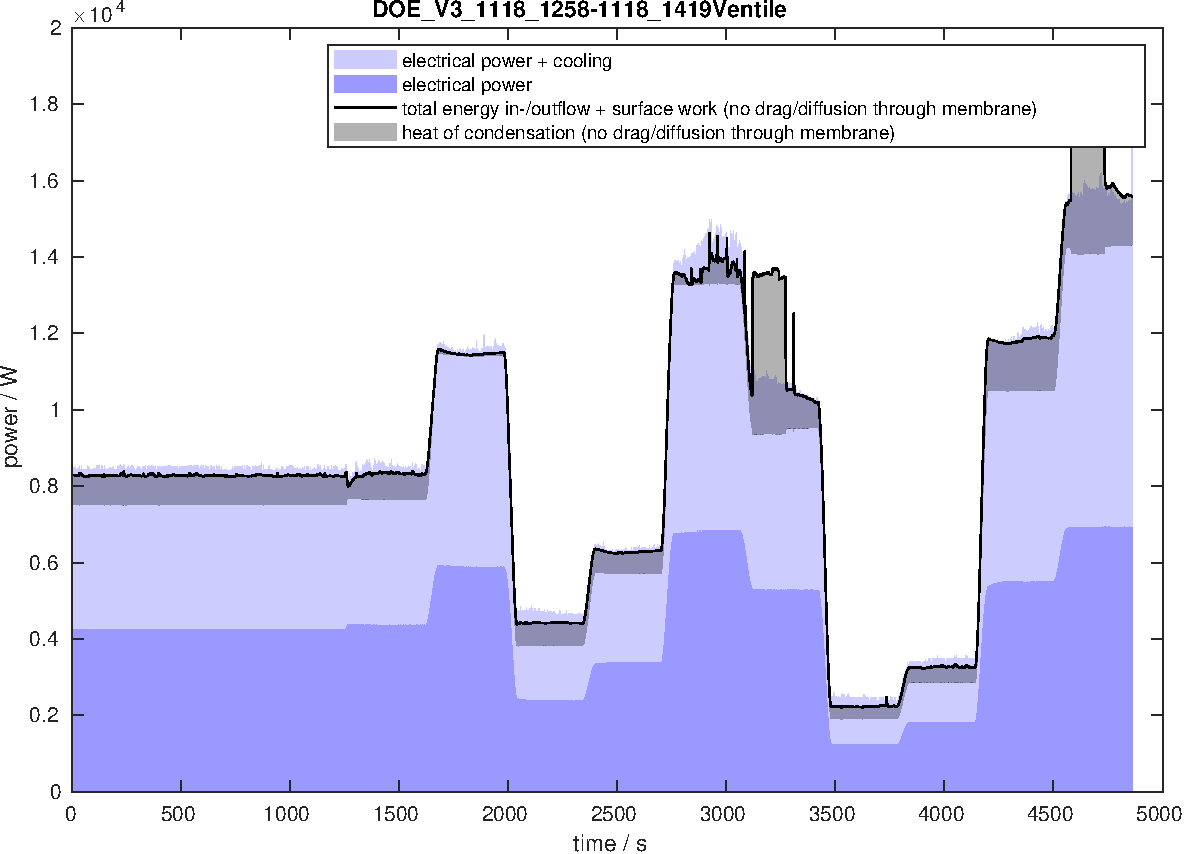
\includegraphics[scale=0.6]{./figures/energyBalance_DoE_v3}
       \end{center}
   %%%
\end{itemize}
%
%
\subsection{Estimation from test bench inputs}
%
If measuremsts from the test bench are not yet available, \eg for the design of a future experiment, the rate of liquid water production can be estimated from fuel cell stack inputs alone by making further assumptions.
The fuel cell voltage and the resulting stack outlet temperature as well as the gas pressures at the inlets are unknown in this case.
Depending on the available knowledge, the cooling outlet temperatures can be estimated from a simplified energy balance.\smallskip
%
\begin{itemize}
   %%%
   \item \highlightg{additional assumptions}
     \begin{itemize}
      \item cooling water and cathode gas in co-flow, anode gas in counter-flow
      \item gas temperatures approach cooling temperature at the gas outlets\\
            $T_\vl{out,c} \approx T_\vl{cool,out}$, $T_\vl{out,a} \approx T_\vl{cool,in}$
      \item options for $T_\vl{cool,out}$
        \begin{itemize} 
          \item $T_\vl{cool,out} \approx T_\vl{cool,in}$ (this overestimates condensation because ${T_\vl{cool,out}\ge T_\vl{cool,in}}$)
          \item assuming a fixed value for the average cell voltage $U_\vl{cell}=\text{constant}$
          \item assuming an average U-I curve for the cell voltage $U_\vl{cell}(I_\vl{cell})$
        \end{itemize}
      \item $p_\vl{in,a/c} \approx p_\vl{out,a/c}$
     \end{itemize}
   %%%
\end{itemize}

%
%% Nomenclature
\newpage
%\fancyhead[ER]{Nomenclature}
%\fancyhead[EL]{\thepage}
%\fancyhead[OR]{\thepage}
%\fancyhead[OL]{Nomenclature}
%
\section{Notation}
\label{section:notation}
%
%

\begin{longtable}	{p{3cm} p{3cm} p{8cm}}
	%
	%
	\textbf{Variables} & ~ & ~ \\
	~ & ~ & ~ \\
	%
	%
	$A$ & $\mathrm{m^2}$ & area \\
	$a$ & $1$ & relative humidity \\
	$C$ & $\mathrm{C ~V^{-1} ~m^{-3}}$ & volumetric capacitance \\
	$c$ & $\mathrm{mol ~m^{-3}}$ & concentration \\
	$c_{\mathrm{p}}$ & $\mathrm{J ~mol^{-1} ~K^{-1}}$ & specific heat capacity \\
	$D$ & $\mathrm{m^2 ~s^{-1}}$ & diffusion coefficient \\
	$e$ & $\mathrm{J ~kg^{-1}}$ & specific total energy \\
	$F$ & $\mathrm{C}$ & Faraday number \\
	$f^{\mathrm{V}}$ & ~ & surface enlargement factor \\
	$h$ & $\mathrm{J ~mol^{-1}}$ & molar enthalpy \\
	$I$ & $\mathrm{A}$ & current \\
	$i$ & $\mathrm{A ~m^{-2}}$ & current density \\
	$L$ & $\mathrm{m}$ & length \\
	$M$ & $\mathrm{kg ~mol^{-1}}$ & molar mass \\
	$\dot{n}$ & $\mathrm{mol ~m^{-2} ~s^{-1}}$ & molar flux density \\
	$P$ & $\mathrm{W}$ & electrical power \\
	$p$ & $\mathrm{Pa}$ & pressure \\
	$R$ & $\mathrm{J ~mol^{-1} K^{-1}}$ & universal gas constant \\
	$r$ & $\mathrm{mol ~m^{-2} ~s^{-1}}$ & reaction rate \\
	$T$ & $\mathrm{K}$ & temperature \\
	$t$ & $\mathrm{s}$ & time \\
	$t_{\mathrm{w}}$ & $~$ & transport number of water in the membrane \\
	$U$ & $\mathrm{V}$ & voltage \\
	$u$ & $\mathrm{J ~kg^{-1}}$ & specific internal energy \\
	$v$ & $\mathrm{m ~s^{-1}}$ & flow velocity \\
	$X$ & $\mathrm{mol ~kg^{-1}}$ & ion exchange capacity \\
	$x$ & $\mathrm{m}$ & space coordinate \\
	$y$ & $\mathrm{m}$ & space coordinate \\
	$z$ & $\mathrm{m}$ & space coordinate \\	
	~ & ~ & ~ \\
	%
	% 
	% 
	%
	$\alpha$ & $\mathrm{W ~m^{-2} ~K^{-1}}$ & heat transfer coefficient \\
	$\delta$ & $\mathrm{m}$ & thickness of layer in $y$-direction \\
	$\kappa$ & $\mathrm{\Omega^{-1} ~m^{-1}}$ & electrical conductivity of the membrane \\
	$\mathit{\Lambda}$ & $~$ & water content \\
	$\lambda$ & $\mathrm{W K^{-1} ~m^{-2}}$ & heat conductivity \\
	$\mu$ & $\mathrm{J mol^{-1}}$ & electrochemical potential \\
	$\xi$ & $~$ & mole fraction \\
	$\rho$ & $\mathrm{kg ~m^{-3}}$ & density \\
	$\mathit{\Phi}$ & $\mathrm{V}$ & electrical potential \\
	~ & ~ & ~ \\
	%
	%
	~ & ~ & ~ \\
	\textbf{Subscripts} & ~ & ~ \\
	~ & ~ & ~ \\
	%
	%
	$\mathrm{A}$ & ~ & anode \\
	$\mathrm{C}$ & ~ & cathode \\
	$\mathrm{CA}$ & ~ & catalyst layer of the anode side \\
	$\mathrm{CC}$ & ~ & catalyst layer of the cathode side \\
	$\mathrm{cool}$ & ~ & cooling \\
	$\mathrm{M}$ & ~ & membrane \\
	$\mathrm{ref}$ & ~ & reference values \\
	$\mathrm{S}$ & ~ & solid \\
	%
\end{longtable}

%
\cleardoublepage
%
\bibliography{ref_PEMFC}
%
%
\end{document}
